\documentclass{article}

% Language setting
% Replace `english' with e.g. `spanish' to change the document language
\usepackage[english]{babel}

% Set page size and margins
% Replace `letterpaper' with `a4paper' for UK/EU standard size
\usepackage[letterpaper,top=2cm,bottom=2cm,left=3cm,right=3cm,marginparwidth=1.75cm]{geometry}
\usepackage{CJKutf8}
% Useful packages
\usepackage{amsmath}
\usepackage{graphicx}
\usepackage{setspace}
\usepackage{float}
\usepackage{subfigure}
\usepackage[section]{placeins}
\usepackage[colorlinks=true, allcolors=blue]{hyperref}
\usepackage[export]{adjustbox}
\usepackage{array}

\author{B10209040 陳彥倫}

\begin{document}
\thispagestyle{empty}
\hfill {\scshape \large Statistics with Meteorological Applications, Spring 2024} \hfill {\scshape P1}
\smallskip
\hrule
\begin{CJK*}{UTF8}{bsmi}
\bigskip
\bigskip
\bigskip

\centerline{\huge \textbf {HW8}}
\bigskip
\centerline{\textbf {B10209040 陳彥倫}}

\bigskip
\bigskip
\bigskip

\section*{8.1}
    \begin{spacing}{2.5}
            \begin{figure}[h]
                \centering
                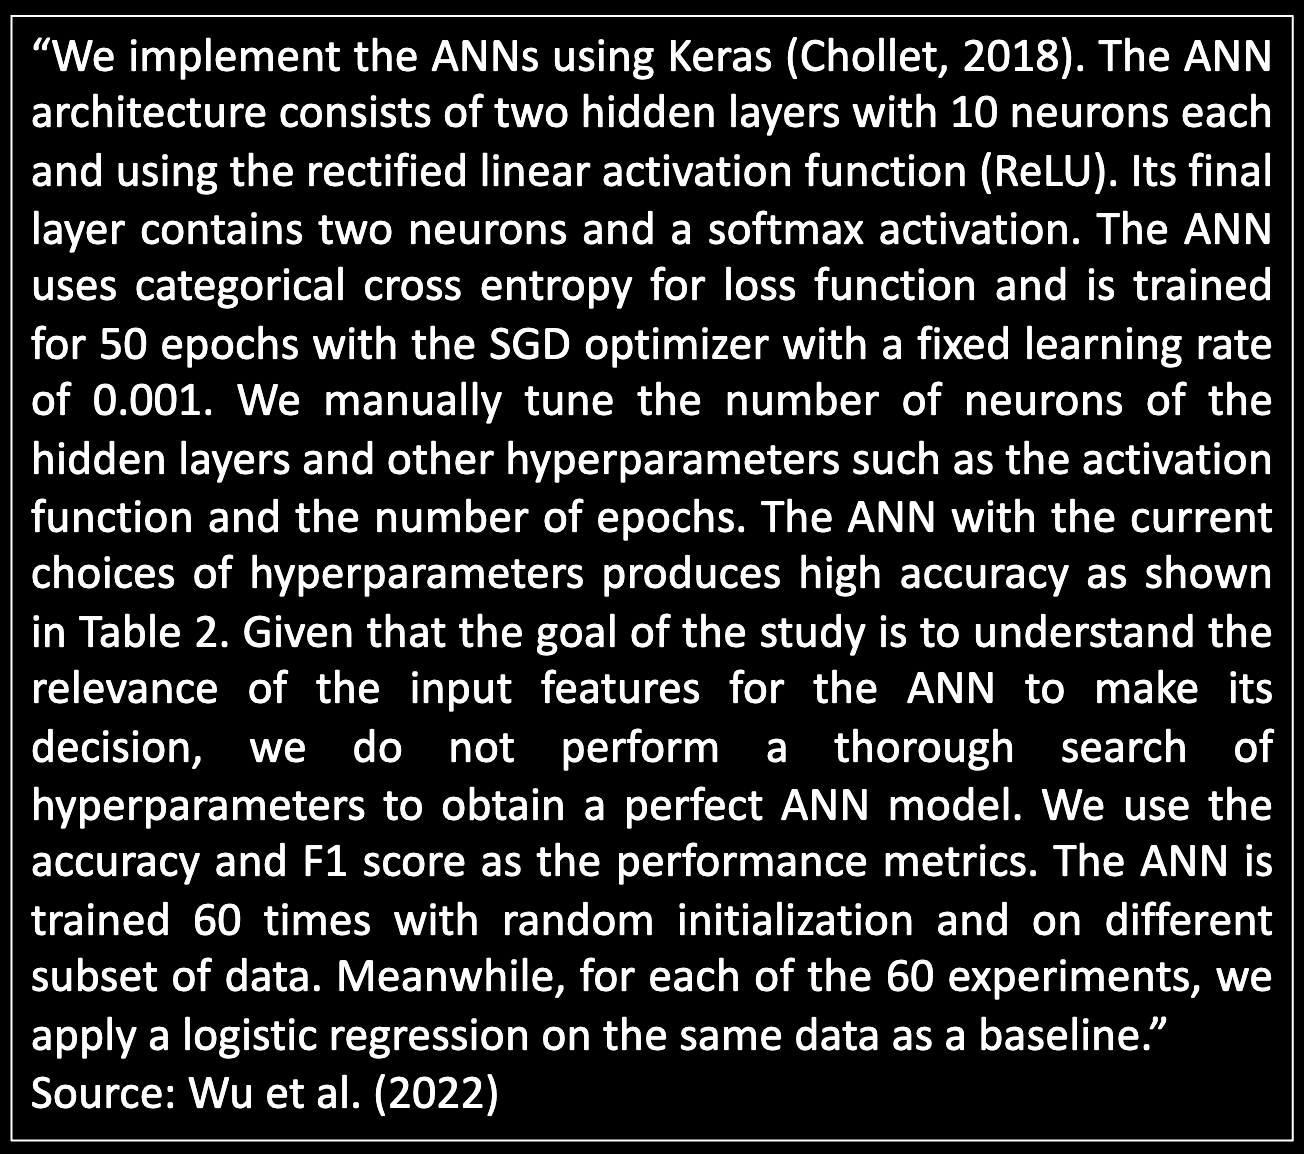
\includegraphics[width=0.7\textwidth]{1.png}
            \end{figure}
        \subsection*{The role of logistic regression:}
            \begin{large}
                A logistic regression model was used as a baseline to compare the ANN's performance, helping to 
                validate the effectiveness of the ANN in handling the given task.
            \end{large}
    \end{spacing}

\newpage
\thispagestyle{empty}
\hfill {\scshape \large Statistics with Meteorological Applications, Spring 2024} \hfill {\scshape P2}
\smallskip
\hrule
\bigskip
\bigskip
\bigskip


\section*{8.2}
    \begin{spacing}{2.5}
        \begin{large}
            \subsection*{1.}
                We use logistic regression model to classify wheather a case is a Sudden Stratospheric Warming
                (SSW) or not. First create training set from 70\% of dataset, and testing set from the rest.
                The input and output sizes of the model are 144 and 1 respectively.
            \subsection*{2.}
            \textbf{Training Loss:} The measure of error or the discrepancy between the model’s predictions and 
            the actual labels during the training phase. \\
            \textbf{Training Accuracy:} The percentage of correct predictions made by the model on the training 
            dataset. It’s a direct indicator of how well the model is learning from the data it is trained on.
            The smaller the better.\\
            \textbf{Testing Loss:} Similar to training loss, this is the measure of error between the model’s pr
            edictions and the actual labels on a new, unseen dataset (the test dataset).\\
            \textbf{Testing Accuracy:} The percentage of correct predictions made by the model on the training 
            dataset. It’s a direct indicator of how well the model is learning from the data it is trained on.
            The smaller the better.\\

        \end{large}
    \end{spacing}

\newpage
\thispagestyle{empty}
\hfill {\scshape \large Statistics with Meteorological Applications, Spring 2024} \hfill {\scshape P3}
\smallskip
\hrule

\subsection*{}
    \begin{spacing}{2.5}
        \begin{large}
            In this case, the training and testing accuracy kept increasing during training. However the train 
            accuracy went up to around 0.9857 and stopped. We can also observe that errors became less as time 
            went on.
            \begin{figure}[h]
                \centering
                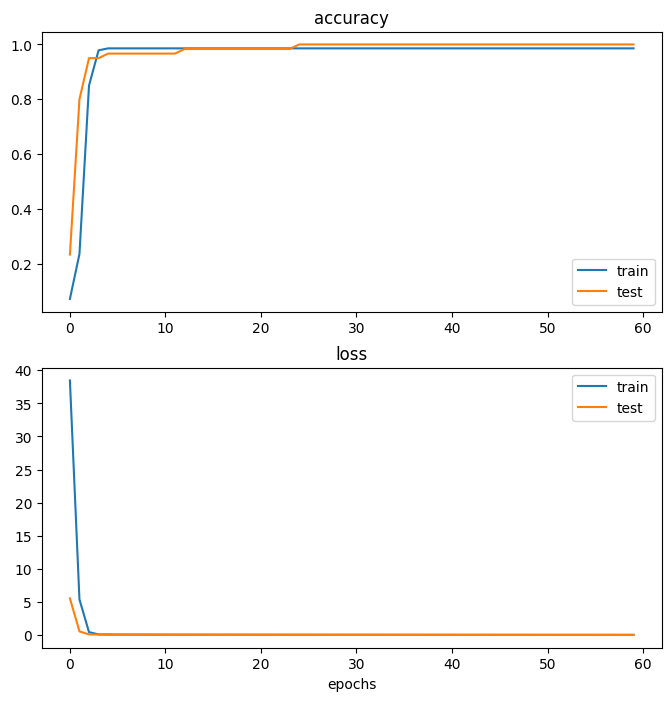
\includegraphics[width=0.7\textwidth]{output1.png}
            \end{figure}
        \end{large}
    \end{spacing}

\end{CJK*}
\end{document}